図\ref{ssr}は8個ロボットの$\theta$(図\ref{course1})と時間の関係図である,
横軸は時間($秒$),縦軸は角度$\theta$である.

\begin{figure}[!ht]
     \centering
     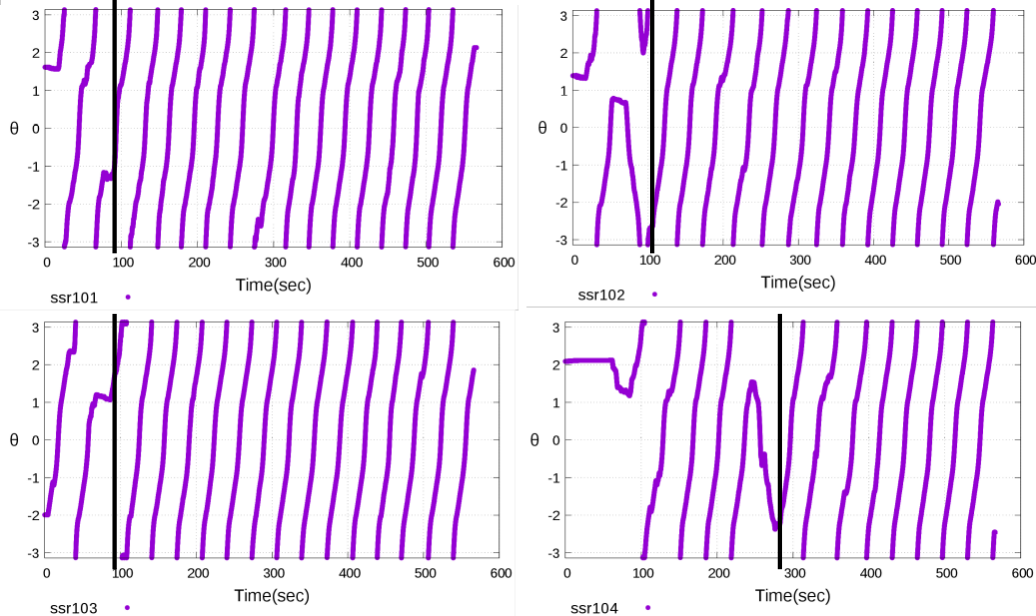
\includegraphics[width=1.0\linewidth]{ssr4_1.png}
\end{figure}

\vspace{-8mm}
\begin{figure}[!ht]\label{ssr2}
     \centering
     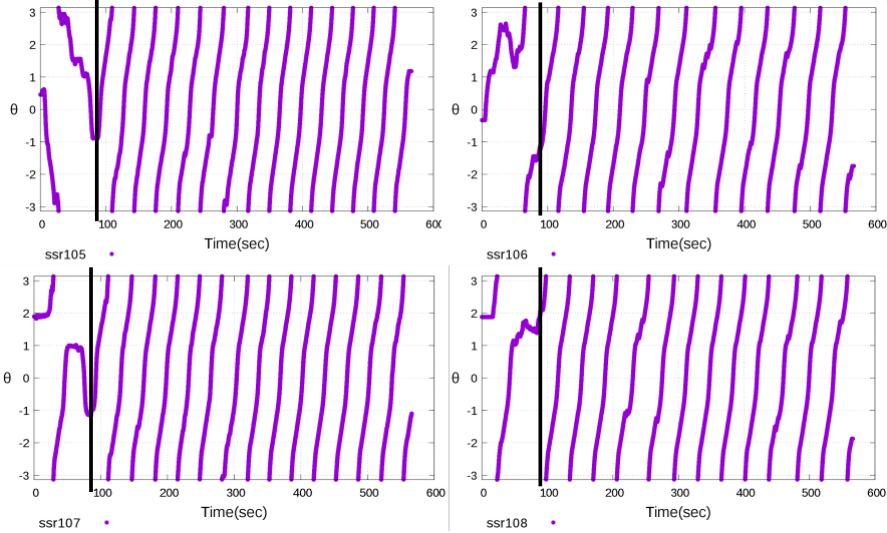
\includegraphics[width=1.0\linewidth]{ssr4_2.png}
     \caption{コース中心から見たロボットの角度$\theta$の時間変化}
     \label{ssr}
\end{figure}


$T_{\rm sd}$とは全てのロボットが方向転換せず,
同じ向きで走る状態になる時間である,
図7中の黒い線はロボットが方向転換しなくなるまでの時間,
その中で一番長いものを$T_{\rm sd}$とする.




